% kelompok 5 
% Adam noerhidayatullah (1174096)
% Sava Reyhano (1174046)
% Faisal Najib Abdullah (1174042)
% Muhammad Lazuardi Habibillah Ritonga (1174061)
% Ihsan Kamal Bangun (1174045)
% M. Athallariq. F (1174055)
% Restiyana Dwi Astuti (1154077)

\section{Implementasi Perangkat Lunak}
Hambatan kinerja dan blok fungsional yang dijelaskan di atas adalah pertimbangan yang diperlukan, namun pada tingkat yang lebih tinggi, masalah implementasi juga harus diperhitungkan. OEM perlu membawa produk mereka ke pasar dengan cepat. Mereka juga harus memastikan bahwa produk ini dapat diupgrade ke versi baru standar ITU V.90 yang mungkin dilepaskan. Implementasi perangkat keras modem V.90 akan jauh lebih sulit untuk diupgrade daripada implementasi perangkat lunak. Implementasi perangkat lunak pada DSP tidak hanya dapat diupgrade; Hal ini juga memungkinkan beberapa fungsi berjalan pada satu prosesor. Ini memberi fleksibilitas pada perancang dalam desain produk dan juga rasio biaya / kinerja yang lebih baik. Begitu keputusan dibuat sesuai dengan implementasi perangkat lunak, OEM harus merancang perangkat lunak itu sendiri atau mengizinkannya. Perangkat lunak modem rumit dan karena itu sulit dikembangkan. Hal ini membutuhkan banyak waktu untuk menciptakan perangkat lunak modem berperforma tinggi dan waktu ke pasar sangat penting dalam industri modem. Jika sebuah produk dilepaskan terlambat, ia akan melewatkan kesempatan pasar yang sempit. Untungnya, ada vendor perangkat lunak seperti GAO Research \& Consulting yang memiliki kode modem berkualitas siap untuk lisensi. Hal ini membuat perangkat lunak perizinan dari vendor menjadi pilihan tercepat dan paling ekonomis bagi OEM yang mengembangkan produk dengan modem V.90.

Karena alasan di atas, minat terhadap implementasi perangkat lunak V.90, serta data pompa modem dan faks lainnya untuk DSP dan mikroprosesor, telah meningkat secara dramatis dalam beberapa tahun terakhir. Dengan meningkatnya popularitas implementasi perangkat lunak teknologi modem dan faks, perancang perlu memahami prinsip operasional dan blok bangunan perangkat lunak modem dan faksimili untuk membuat keputusan terdidik tentang perizinan perangkat lunak ini.

\section{Abstract}
Modem subscriber analog berkecepatan tinggi beroperasi pada kecepatan setinggi 64 kbps baik pada arah downlink maupun uplink menggunakan garis POTS standar ditambah dengan codec yang disempurnakan. Hal ini memungkinkan peningkatan kecepatan upload dan mendukung koneksi pelanggan analog peer-to-peer 56 kbps. Sebuah codec jaringan yang disempurnakan sesuai dengan penemuan ini mendukung jalur POTS baik komunikasi modem berkecepatan tinggi maupun komunikasi ucapan PCM standar.

\section{definisi}
Modem 56K yang terlihat seperti gambar \ref{modem56k} diperkenalkan di bawah dua standar bersaing yang tidak sesuai. pentingnya persaingan antara penyedia layanan internet dalam proses adopsi.
Bahwa ISP, cenderung mengadopsi teknologi yang lebih banyak pesaing . Hasil ini sangat mencolok mengingat peserta industri mengharapkan koordinasi dalam satu standar atau yang lain.
Berspekulasi tentang peran diferensiasi ISP dalam mencegah pasar mencapai standardisasi sampai organisasi pengaturan standar ikut campur.
Materi pokok dari aplikasi ini terkait erat dengan aplikasi copending berikut yang berhubungan dengan aspek-aspek tertentu dari penemuan ini seperti yang diungkapkan disini dan digabungkan disini sebagai referensi: ``Modem kecepatan tinggi dengan pencoba echo-downlink jauh,'' nomor seri tidak diketahui, oleh Eric M. Dowling dan mengajukan permohonan pada hari yang sama dengan aplikasi ini, 14 Januari 1999.
\begin{figure}[ht]
	\centerline{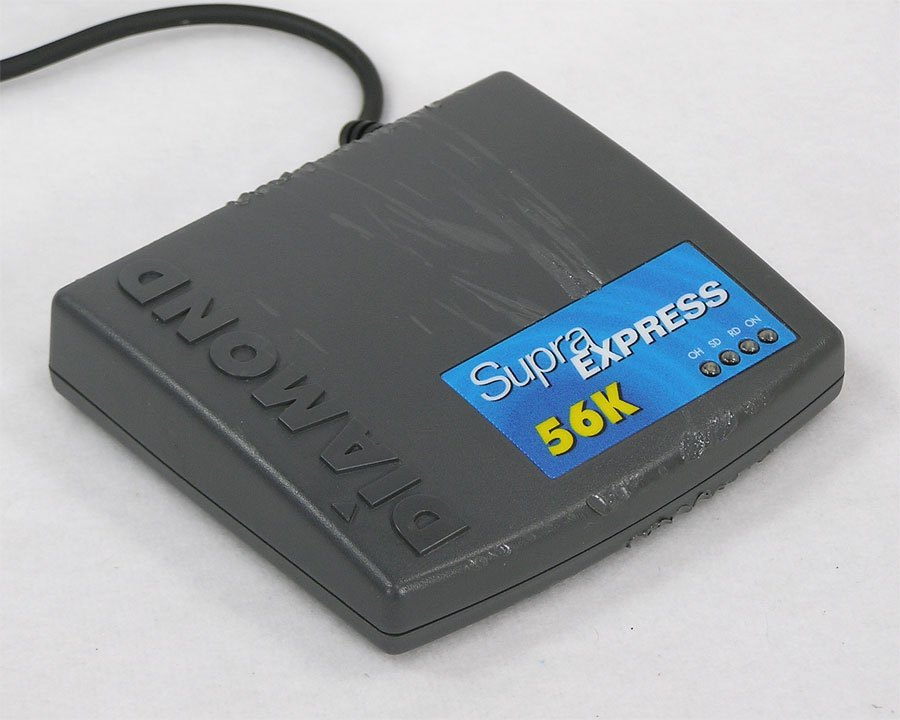
\includegraphics[width=1\textwidth]{figures/modem56k.jpg}}
	\caption{modem 56k}
	\label{modem56k}
	\end{figure}
	
\subsection{Introduction} Modem V.90 adalah teknologi terbaru yang menawarkan kecepatan koneksi Internet lebih cepat tanpa mengharuskan konsumen berlangganan layanan garis digital yang lebih mahal. Sebelum teknologi V.90, modem secara teoritis dibatasi sekitar 35 Kbps oleh noise kuantisasi yang mempengaruhi konversi analog ke digital (batas praktisnya sebenarnya 33,6 Kbps). Namun, di dunia sekarang ini, dengan meningkatnya fasilitas transmisi digital, aman untuk mengasumsikan bahwa semakin banyak penyedia layanan Internet (ISP) terhubung secara digital baik ke Internet maupun ke kantor pusat perusahaan telepon genggam (KC). Jika demikian, ada koneksi digital yang jelas ke hilir dari modem ISP ke kartu jalur CO yang melayani pengguna dan berisi konverter digital ke analog. Hasil dari koneksi digital ini adalah bahwa konversi analog ke digital (dan oleh karena itu kebisingan kuantisasi) dapat dihindari antara ISP dan CO. Tanpa batasan yang diberlakukan oleh kebisingan kuantisasi, secara teoritis dimungkinkan untuk mencapai kecepatan koneksi hilir hingga 64 Kbps. Praktis, bagaimanapun, ini belum mungkin dilakukan. Hambatan kinerja seperti kuantisasi μ-law mengurangi laju data efektif modem V.90 hingga maksimum 56 Kbps downstream.

Di arah hilir, modem V.90 beroperasi menggunakan modulasi amplitudo pulsa (PAM). Sinyal hilir terdiri dari 8000 simbol per detik dan setiap simbol secara maksimal dikodekan dari 7 bit masing-masing kata kode modulasi kode 8-bit (PCM). Ini berarti 128 tingkat amplitudo yang mungkin ada dalam sinyal PAM. Karena sebagian besar pengguna tidak terhubung secara digital dengan CO, sebuah konversi analog-ke-digital dan noise kuantisasi terkait tidak dapat dihindari pada arah hulu. Ini berarti bahwa teknik modulasi V.34 harus digunakan dan kecepatan hulu masih terbatas pada 33,6 Kbps. Gambar 1 dan 2 mengilustrasikan konfigurasi dasar modem V.90 dan modem klien (arah hilir) seperti yang ditentukan oleh standar International Telecommunications Union (ITU) V.90.
Karena standar V.90 baru saja selesai pada akhir September 1998, artikel ini memberikan gambaran tepat waktu tentang standar modem, fungsi pemancar dan penerima V.90, hambatan terhadap kinerja, dan implementasi perangkat lunak. Gambaran ini harus membantu desainer membuat keputusan terdidik tentang merancang produk dengan model modem V.90.

Standar V.90 yang telah diratifikasi mendefinisikan karakteristik utama modem 56K sebagai berikut: 
\begin{itemize}
\item Mode operasi dupleks melalui jaringan telepon tetap (PSTN) dan jaringan digital yang diaktifkan. Penggunaan teknik pembatalan gema untuk pemisahan saluran. Modulasi PCM ke hilir pada tingkat simbol 8 k dan modulasi V.34 hulu.
\item Tingkat sinyal data kanal sinkron turun dari 28 Kbps menjadi 56 Kbps dengan penambahan 1,3 Kbps dan hulu dari 4,8 Kbps menjadi 33,6 Kbps dengan penambahan 2,4 Kbps.
\item Modem menggunakan teknik adaptif untuk mencapai sedekat mungkin dengan tingkat sinyal data maksimum yang didukung oleh saluran pada setiap koneksi. 
\item Jika sambungan tidak mendukung V.90, modem jatuh kembali ke operasi V.34 dupleks penuh. Selama dimulainya modem, laju sinyal data ditetapkan dengan urutan nilai tukar.
\item Prosedur automode V.32bis dan mesin faksimili Grup 3 mendukung modem Automoding ke V.Series. 
\item V.8 dan secara opsional, prosedur V.8bis tersedia saat start up modem atau seleksi. \cite{gao1998introduction} 
\end{itemize}
\section{sejarah}
Penemuan ini memecahkan sebuah masalah dengan menyediakan sistem dan metode untuk memungkinkan koneksi modem simetris berkecepatan tinggi antara modem digital dan analog atau pelanggan modem analog. Codec PCM yang disempurnakan dengan kemampuan pemrosesan sinyal digital dikembangkan untuk memungkinkan uplink dioperasikan 56 kbps atau sampai 64 kbps dalam beberapa kasus. Codec jaringan yang disempurnakan membatalkan gema seperti yang terlihat pada input ADC 140 codec pada jaringan. Salah satu aspek dari penemuan ini menggabungkan struktur pembatalan gema ke dalam arsitektur codec PCM yang disempurnakan. Kemampuan penerima sinyal uplink dibangun ke dalam codec PCM yang disempurnakan agar memungkinkan untuk memproses sinyal modem uplink baik dan kecepatan tinggi (misalnya, 56 kbps). Codec PCM yang disempurnakan dari penemuan ini dapat diwujudkan pada mati semikonduktor tunggal dan dikemas agar sesuai dengan codec yang ada. Ini memungkinkan kartu antarmuka jaringan yang ada untuk ditingkatkan dengan biaya dan upaya minimum untuk membuat antarmuka jaringan yang disempurnakan yang mampu mendukung lalu lintas bi kiper directional 56 kbps. Modem bidirectional 56 kbps yang ditingkatkan untuk penggunaan dengan codec PCM yang disempurnakan dan prosedur pelatihan kooperatif terkait juga dikembangkan
Dalam aspek pertama dari penemuan ini, aparatus codec yang disempurnakan untuk digunakan dalam kartu antarmuka jaringan dikembangkan. Aparatus ini mencakup sirkuit prosesor sinyal digital, dan port antarmuka digital dengan kopling pertama ke sirkuit prosesor sinyal digital dan kopling kedua ke jaringan digital.
Aspek kedua dari penemuan ini berfokus pada peralatan codec lain yang disempurnakan. Aparatus ini termasuk DAC, dan sebuah ADC. Codec yang disempurnakan juga menyertakan modul fungsi pemetaan. Pembatalan gema juga disertakan yang berfungsi untuk membatalkan komponen gema yang bocor dari keluaran analog DAC kembali ke input analog ADC melalui, misalnya, antarmuka. Modul fungsi pemetaan berfungsi untuk secara selektif mengubah representasi digital dari sinyal analog uplink ke salah satu representasi bentuk gelombang PCM dan aliran bit yang didekode yang dimasukkan ke dalam aliran data PCM.
Aspek ketiga dari penemuan ini, berhubungan dengan modem pelanggan yang dapat dipasangkan pada saluran POTS dari jalur pelanggan dan dioperasikan untuk berkomunikasi dengan codec yang disempurnakan.
Aspek keempat dari penemuan ini membahas metode pengolahan untuk penggunaan dalam codec yang disempurnakan.
Jadi Dalam metode ini, aliran data berkecepatan tinggi diekstraksi dari bentuk gelombang uplink-analog, yang dikodekan ke dalam aliran data PCM, dan dikirim ke jaringan digital. Aspek lain dari penemuan ini menangani metode serupa yang dilakukan di modem pelanggan saat berkomunikasi dengan codec yang disempurnakan.

Implementasi Perangkat Lunak
Hambatan kinerja dan blok fungsional yang dijelaskan di atas adalah pertimbangan yang diperlukan, namun pada tingkat yang lebih tinggi, masalah implementasi juga harus diperhitungkan. OEM perlu membawa produk mereka ke pasar dengan cepat. Mereka juga harus memastikan bahwa produk ini dapat diupgrade ke versi baru standar ITU V.90 yang mungkin dilepaskan. Implementasi perangkat keras modem V.90 akan jauh lebih sulit untuk diupgrade daripada implementasi perangkat lunak. Implementasi perangkat lunak pada DSP tidak hanya dapat diupgrade; Hal ini juga memungkinkan beberapa fungsi berjalan pada satu prosesor. Ini memberi fleksibilitas pada perancang dalam desain produk dan juga rasio biaya / kinerja yang lebih baik. Begitu keputusan dibuat sesuai dengan implementasi perangkat lunak, OEM harus merancang perangkat lunak itu sendiri atau mengizinkannya. Perangkat lunak modem rumit dan karena itu sulit dikembangkan. Hal ini membutuhkan banyak waktu untuk menciptakan perangkat lunak modem berperforma tinggi dan waktu ke pasar sangat penting dalam industri modem. Jika sebuah produk dilepaskan terlambat, ia akan melewatkan kesempatan pasar yang sempit. Untungnya, ada vendor perangkat lunak seperti GAO Research \& Consulting yang memiliki kode modem berkualitas siap untuk lisensi. Hal ini membuat perangkat lunak perizinan dari vendor menjadi pilihan tercepat dan paling ekonomis bagi OEM yang mengembangkan produk dengan modem V.90.

Karena alasan di atas, minat terhadap implementasi perangkat lunak V.90, serta data pompa modem dan faks lainnya untuk DSP dan mikroprosesor, telah meningkat secara dramatis dalam beberapa tahun terakhir. Dengan meningkatnya popularitas implementasi perangkat lunak teknologi modem dan faks, perancang perlu memahami prinsip operasional dan blok bangunan perangkat lunak modem dan faksimili untuk membuat keputusan terdidik tentang perizinan perangkat lunak ini.

\section {karakteristik}
Karakteristik yang harus dicari jika Anda lisensi V.90 perangkat lunak:
\begin{enumerate}
\item Harus sesuai dengan standar ITU V.90.
\item Perangkat lunak harus diuji sesuai standar.
\item Harus mengambil jumlah memori terkecil dan MIPS.
\item Vendor harus memiliki reputasi yang baik untuk kualitas.
\item Vendor harus memberikan dukungan yang baik karena software ini sangat kompleks dan tergantung hardware.
\end{enumerate}
\section{Ringkasan}

Modem V.90 adalah kemajuan teknis nan inovatif, yang memperluas kemampuan analog untuk meningkatkan kecepatan aplikasi Internet. Teknologi modem baru ini memanfaatkan teknik pengkodean dan pengodingan yang canggih, namun masih banyak hambatan kinerja yang harus diatasi oleh perancang modem V.90 agar bisa memberikan kecepatan data hingga 56 Kbps. Seperti implementasi modem pra standar lainnya, ada masalah kompatibilitas serius antara teknologi yang bersaing, namun ini telah diselesaikan dengan standar V.90. Karena standarnya sangat baru, modem V.90 harus bisa upgrade ke versi baru. Cara terbaik untuk memastikan upgrade yang mudah adalah dengan menerapkan modem berbasis perangkat lunak daripada modem berbasis chipset perangkat keras. Selanjutnya, modem berbasis software menawarkan waktu yang lebih cepat ke pasar dan rasio biaya kinerja yang lebih baik di sebagian besar aplikasi.

\section{kesimpulan}

Dalam penjelasan diatas, modem 56k sangatlah diperlukan dalam mengakses internet. Kita harus berterima kasih kepada pencipta modem 56k. Karena kalau tidak ada dia maka kita tidak akan bisa melakukan chatting di berbagai sosmed dengan cepat. Dialah Dennis Heyes pencipta modem dengan kecepatan 56k. Apalagi ada perbedaan dalam modem 56k antara v90 dengan v92. Dengan penggunaan modem dapat mengurangi kerumitan dan kesalah dalam penggunaan komputer yg mempunyai jalur komunikasi dua arah. Sekian artikel ini kami buat. Wassalamualaikum warahmatullahi wabarokatuh
